
\documentclass{article}

\usepackage{amsmath}
\usepackage[utf8]{inputenc}
\usepackage[a4paper]{geometry}
\usepackage[shortlabels]{enumitem}
\usepackage{graphicx}

\graphicspath{ {../assets/} }

\makeatletter
\renewcommand{\@seccntformat}[1]{}
\makeatother

\makeatletter
\newcommand*{\rom}[1]{\expandafter\@slowromancap\romannumeral #1@}
\makeatother

\setlength\parindent{0pt}

\title{Werkstoffe und Fertigung \rom{1} - Notizen}
\author{Ahmed Bajra}
\date{2020-09-20}

\begin{document}
\maketitle

\section{Intro}
\subsection{Weitere Beispiele für Produktionsinnovation}
\begin{itemize}
    \item "Stahlbanane"
\end{itemize} 

Verformarkeit und Festigkeit sind in negativer Abhängigkeit bei Werkstoffen

\begin{itemize}
    \item Ultra Light Steel Body (ULSB) $\rightarrow$ Versuch der Stahlproduktion, Aluminium konkurrenz zu machen mit leichter \textbf{Autokarrosserie}
\end{itemize}

Werkstoffeigenschaften:
\begin{itemize}
    \item Gebrauchseigenschaften
    \item Fertigungseigenschaften
    \item Komerzielle Eigenschaften (Kosten)
    \item Umwelteigenschaften
\end{itemize}

\subsection{Kommerzielle Eigenschaften}

Der billigste, gerade noch geeignete Werkstoff ist zu Wählen
\[
    \frac{G + F}{P}=max.
\]

G = Mass für Gebrauchseigenschaften
F = Mass für Fertigungseigenschaften
P = Preis

\newpage

\subsubsection{Umwelteigenschaften}

\begin{itemize}
    \item Umweltbelastung
    \item Toxizität
    \item Wasserverbrauch
    \item Energieverbrauch bei Herstellung
    \item Recyclingfähigkeit 

    \item Sorteinreine Trennung
    \item Degradation
    \item Begleitelemente - Bsp.: Wiederverwendung von Stahl aus der Autoproduktion verunreinigte mit \textbf{Kupfer}
    \item Ministahlwerke
\end{itemize}

Ziel: Wenig entsorgen, mehr recycling - "Stoffkreisläufe schliessen"

Werkstoff der Zukunft: Keramik

\subsection{Werkstoff(haupt)gruppen}
\begin{itemize}
    \item Metalle (M)
    \item Polymere (P)
    \item Keramik / Gläser (K)
    \item Verbundstoffe (V)
\end{itemize}

M + K $\rightarrow$ Halbleiter, Supraleiter

M + P $\rightarrow$ Leitfähige Polymere

K + P $\rightarrow$ Silikone

\newpage

\subsubsection{Cremeschnitte}
Ziel: Cremeschnitten für ganze Stadt Zürich portionieren, Messer geht nicht

Mittel: Wasserstrahlschneider

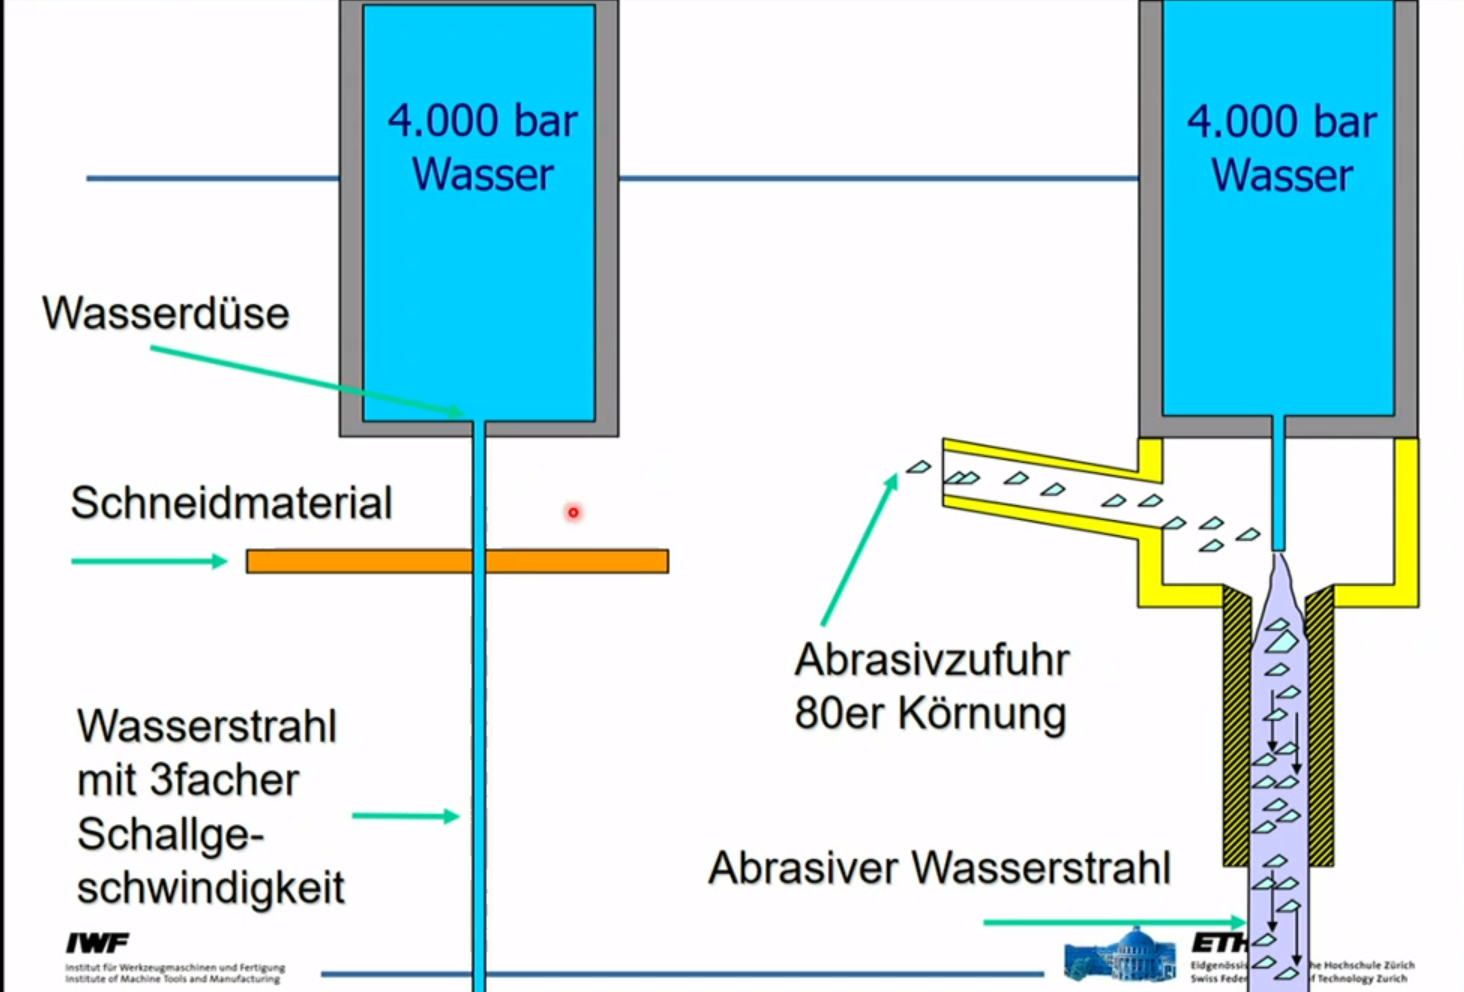
\includegraphics[scale=0.25]{wasserstrahl-09-21}


\end{document}